\section{SIM TIPS Simulator}

TIPS (Tips Is a Pixel Simulator) is mainly written in Python, but its core is based on aXeSIM, which is written in C and then wrapped in python by TIPS itself. The TIPS official gitlab repository can be found at the link

\begin{center}
\url{https://gitlab.euclid-sgs.uk/PF-SIM/SIM_TIPS_Simulator}    
\end{center}

Essentially TIPS has three main programs:

\begin{itemize}
\item \verb+EuclidNisSplit.py+: it creates the TIPS fits configuration and catalog files;
\item \verb+EuclidNisDetector.py+: it performs the pixel simulation at the single detector level, taking the configuration and catalog files as inputs;
\item \verb+EuclidNisCombine.py+: it takes all the 16 detector simulated frames and combines them into a single fits file.
\end{itemize}

\begin{figure}
    \centering
    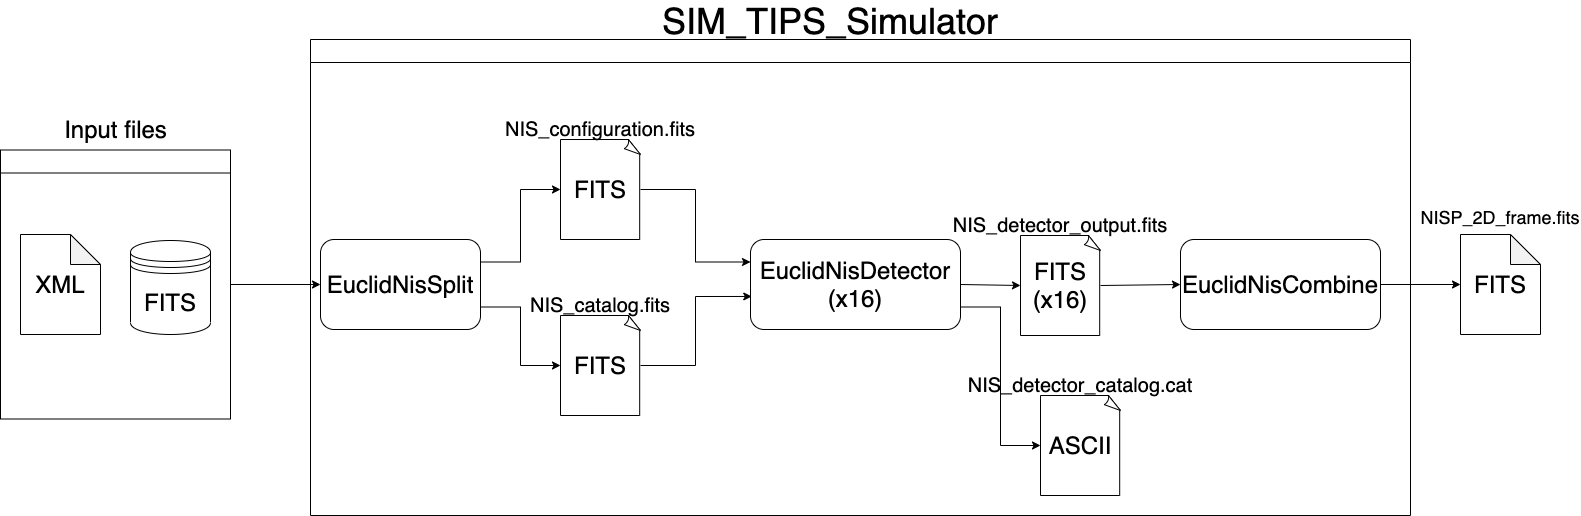
\includegraphics[scale=0.25]{figures/TIPS_workflow.png}
    \caption{Schematic representation of the workflow of TIPS.}
    \label{fig:TIPS_workflow}
\end{figure}

In the next section we describe the necessary input files for a TIPS simulation.

\subsection{TIPS input files}
In plain words, what TIPS needs to run a simulation can be summarized as follows:

\begin{itemize}
\item The catalogs of the sources (stars and galaxies) whose 2D spectra are to be simulated, optionally along with their spectra
\item The instrument and telescope configurations: i.e. the active instrumental effects, the grism used, the pointing coordinates, etc \dots
\item The Euclid Mission configuration, i.e. the Mission Database (MDB).
\end{itemize}

As shown in \figref{fig:TIPS_workflow} the input files needed for TIPS are essentially XML and FITS files. In particular, the input files passed explicitly as  parameters to TIPS programs are XML files, some of them referencing the other input FITS files. In what follows we give the details of our knowledge about the essential input files.

\subsubsection{XML input files}
Each of these files is a so-called \emph{DataProduct}, i.e. a file which must have a precise format, maintained along with a specific software library of classes to be read and written properly. In fact Data Products are the way with which the often the various Euclid Processing Functions (PFs) and Organization Units (OUs) exchange data. For example a specific DataProduct can be the output, and so there must be a way to 


\paragraph{DpdNisInputConfiguratiom}

The XML input files are the following:

\begin{itemize}
\item \verb+DpdNisInputConfiguration+: the file describing the instrumental configuration to be used;
\item \verb+DpdTrueUniverseOutput+: a file containing the reference to the FITS catalog and spectra files
\item \verb+MissionDataBaseSetOfParameters+: a very big XML file describing the Euclid Mission configuration, as well as many references to FITS input files
\item \verb++
\end{itemize}
